\section{Teknologi} % (fold)
\label{sec:Teknologi}

I dette afsnit bliver forskellige eksisterende teknologier bearbejdet med henblik på at give et overblik. Hver teknologi vil blive introduceret kort, hvorefter styrker og svagheder vil blive præsenteret. Dette kan senere bruges når en løsning skal designes.


\subsection{Navision} % (fold)
\label{sub:Navision}

Navision eller Microsoft Dynamics NAV er et dansk software regnskabsprogram. Det blev oprindeligt udviklet af Jesper Balser, Torben Wind og Peter Bang tilbage i 1984. Siden da har det haft forskellige navne. I 2002 opkøbte Microsoft programmet, og integrede det i deres Microsoft Business Solutions program \cite{visiondata}.

Programmet samler en virksomheds aktiver i en grafisk brugerflade, der gør det enkelt at manipulere data som f.eks.\ medlemmer, materialer og økonomi. Navision er designet til at kunne håndtere alle typer virksomheder, og kan skræddersyes efter behov ved tekniker besøg.

\begin{figure}
  \centering
  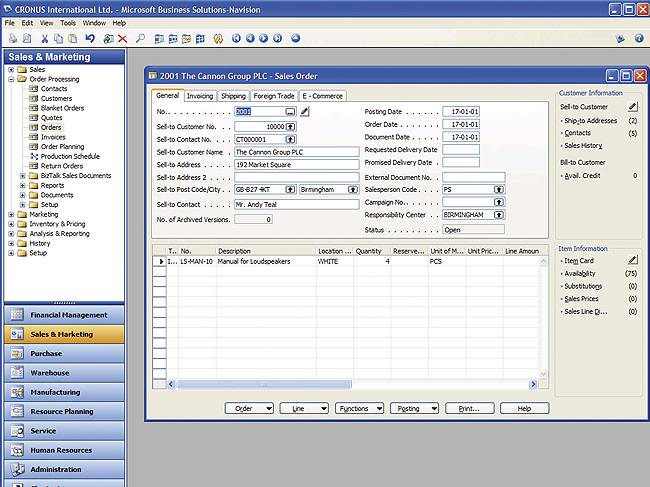
\includegraphics[width=\textwidth]{navision_program.jpg}
  \caption{Eksempel på Navision program-konfiguration - fra \url{http://www.microsoft.com/business/imagelibrary/businesssolutions/ScreenShotImages/mbs_navision_main_menu_sales.jpg}}
  \label{fig:navision_program}
\end{figure}


\sinote{overvej flere problemer, eller omskriv til ental}
Nogle af problemerne med Navision er ifølge Vestre Baadelaug, at man ikke kan lave en regning og sende denne via e-mail \cite{int_vb_sl}. Dette kan dog som tidligere nævnt udbredres ved betaling til supporterende leverandør af Navision.


\subsection{Chip-system} % (fold)
\label{sub:Chip}


chipsystem til faciliteter \& strøm samt parkering

\subsection{Håndtering af gæster - havnefogeden} % (fold)
\label{sub:havnefogeden}

\sinote{Mangler info fra havnefogeden}


\subsection{MarinaBooking.dk} % (fold)
\label{sub:MarinaBooking.dk}

Formålet med MarinaBooking \cite{marinabooking} er at gøre vandpladsreservationer lettere for gæster til lystbådehavne i Danmark. Systemet fungerer ved at gæster indtaster ankomst- samt afgangsdato, hvilken havn de vil lægge til og deres båds dimensioner. MarinaBooking kan med disse informationer nu præsentere et oversigtskort over havnebroerne på den specificerede havn, hvor gæsten kan vælge den ønskede vandplads på kortet. Systemet opkræver betaling, og gæsten har nu reserveret denne vandplads.

For at MarinaBooking kan fungere, skal lystbådehavne aktivt tilmelde sig. Dette kan ikke alle havne gøre, f.eks.\ fordi de ikke har en bro udelukkende til gæster  \sinote(link til hvor vi skriver om VB's layout angående gæster/medlemsbro). 

MarinaBooking gør det enkelt for gæster fra Danmark, såvel som fra udlandet, at bestille havepladser fra internettet. Dette er godt for gæsterne, men også for administrationen i havnen, da tildeling af vandpladser herved ordner sig selv.

En af ulemperne ved MarinaBooking er det begrænsede udvalg af samarbejdshavne på hjemmesiden. Dette kan blandt andet skyldes ovenstående forklaring mht.\ gæstebroer.


\subsection{E-conomic} % (fold)
\label{sub:e-conomic}

E-conomic er både navnet på en virksomhed og deres online regnskabsprogram. Formålet med programmet er at gøre økomnomi-håndtering let for selv ikke-regnskabsuddannede. E-conomic henvender sig primært til små- og mellemstore virksomheder \cite{economic}. Prisen for benyttelsen af E-conomic er abonnomentsbaseret med forskellige muligheder for tilpasninger. Da E-conomic kører online i en webbrowser, er alt data gemt og sikkerhedskopieret af E-conomic. Kunden ejer alt data med mulighed for eksportering efter abonnomentsophør.

Fordelene ved e-conomic er den intuitive brugergrænseflade som letter mange bogførings handlinger. Derudover er programmet skrevet som et web-program hvilket gør at det kan tilgås fra alle platforme samt fra mange lokationer.

\begin{figure}
  \centering
  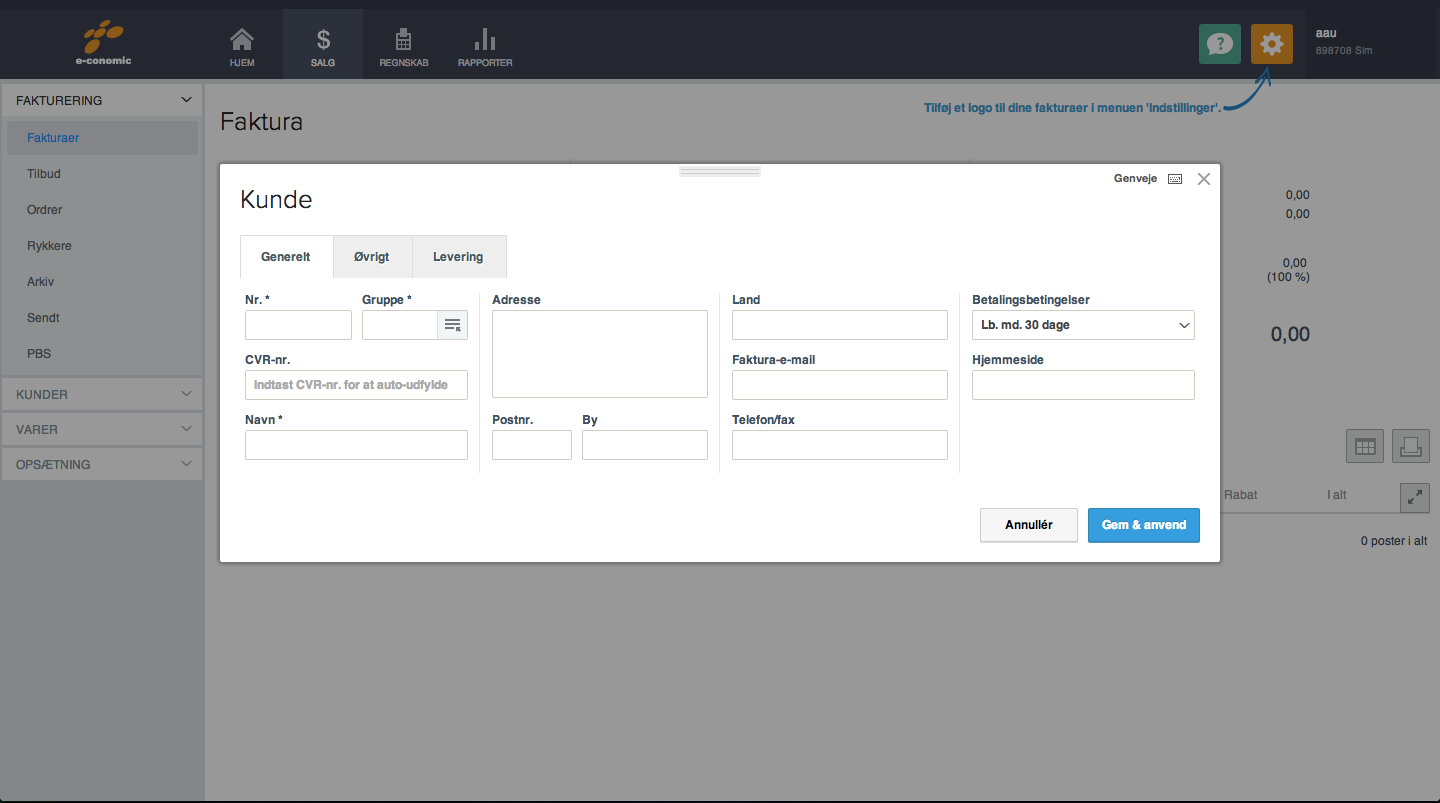
\includegraphics[width=\textwidth]{e-conomic.png}
  \caption{Brugerinterface ved oprettelse af ny faktura - E-conomic}
  \label{fig:e_conomic}
\end{figure}


Ulemperne ved e-conomic inkluderer afhængigheden af E-conomic med dertilhørende risiko for nedetid. 


\subsection{ForeningLet} % (fold)
\label{sub:ForeningLet}

ForeningLet er et online medlemssystem udviklet af Enteleki. Programmet har, som navnet antyder, specialiseret sig i systemer til foreninger. Det kan blandt andet håndtere medlemmer, regnskab, kontingent opkrævninger og bookning af materialer. Den årlige pris for programmet er afhængigt af antallet af medlemmer i foreningen, og desuden koster tillægsmoduler og dertilhørende ydelser ekstra. F.eks.\ koster et opkrævningsmodul 600 kr./år. Dertil kommer et tillæg på 80 øre per dannet opkrævning. I denne årlige pris er hosting, opdatering og vedligeholdelse inkluderet. ForeningLet holder altså styr på alle medlemsdata og gemmer dette på deres servere \cite{foreninglet}.

Navigationen i programmet foretages i en intuitiv brugerflade i en webbrowser. Man kan altså tilgå programmet på en hvilken som helst enhed med internetforbindelse. 

\begin{figure}
  \centering
  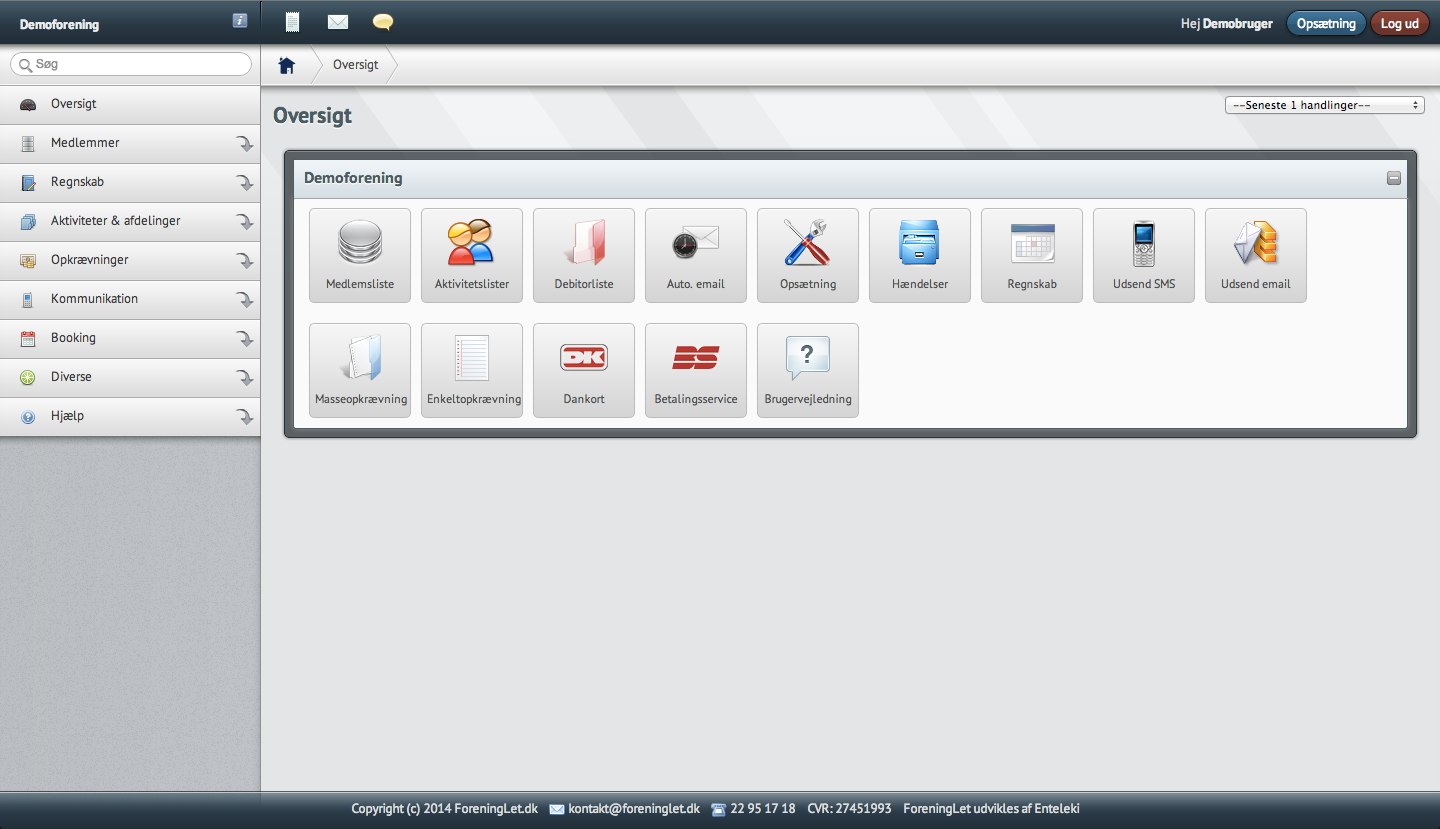
\includegraphics[width=\textwidth]{foreninglet.png}
  \caption{Oversigt over brugergrænsefladen i ForeningLet}
  \label{fig:foreninglet_program}
\end{figure}

Selvom ForeningLet systemet er meget nemt at bruge samt at sætte op, kan man forestille sig at systemet vil være for dyrt for foreninger med mange medlemmer. Dette skyldes førnævnte gebyrer på tillægsydelser som opkrævninger og rykkere. Derudover er foreningen afgængig af ForeningLet på samme måde som beskrevet i \cref{sub:e-conomic}.

% subsection ForeningLet (end)

% section Teknologi (end)
